% Worked MaxCut example of notebook 45c, Section 3.2: the house graph, N = 5, edges 01, 12, 23, 03, 04, 14
% (square 0-1-2-3 with the roof vertex 4 on the edge 01; triangle 0-1-4).
% Left: red group {0,1}, bits s = 11000, cut edges 12, 03, 04, 14 -> P = 4.
% Right: red group {0,2}, bits s = 10100, cut edges 01, 12, 23, 03, 04 -> P = 5 = P_max (only 14 uncut).
% Red vertex: s_i = 1, z_i = -1; white vertex: s_i = 0, z_i = +1.  Cut edges dashed orange, uncut edges solid black.
\documentclass[tikz,border=6pt]{standalone}
\usepackage{amsmath,amssymb}
\usetikzlibrary{calc}
\begin{document}
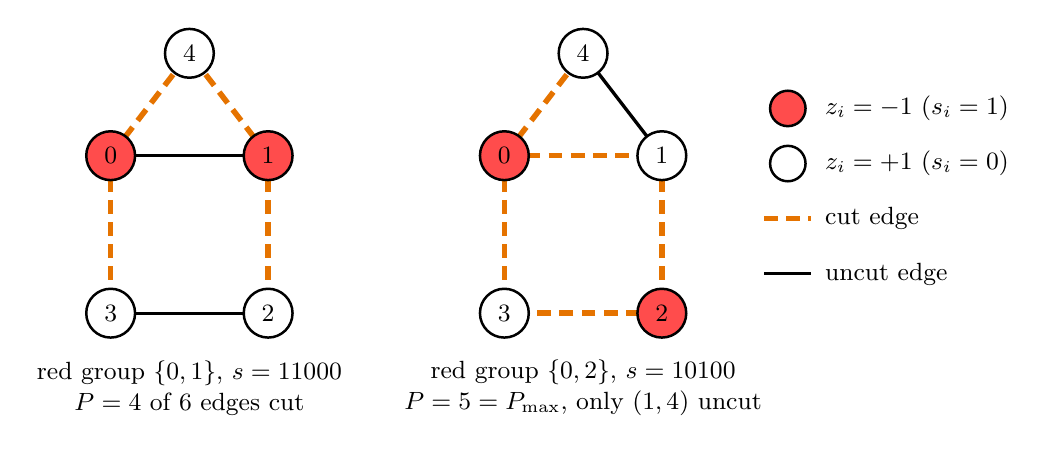
\begin{tikzpicture}[x=1cm, y=1cm,
    uncut/.style={line width=1.2pt, black},
    cutedge/.style={line width=2.0pt, orange!90!black, dash pattern=on 5pt off 3pt},
    vtx/.style={circle, draw=black, line width=0.9pt, minimum size=0.62cm, inner sep=0pt, font=\small}]
  % \house{x}: coordinates a0..a4 of the five vertices, shifted by x
  \newcommand{\house}[1]{%
    \begin{scope}[shift={(#1,0)}]
      \coordinate (a0) at (0,2); \coordinate (a1) at (2,2); \coordinate (a2) at (2,0);
      \coordinate (a3) at (0,0); \coordinate (a4) at (1,3.3);
    \end{scope}}
  % ---------------- left panel: red group {0,1}, P = 4 ----------------
  \house{0}
  \draw[uncut]   (a0) -- (a1);
  \draw[cutedge] (a1) -- (a2);
  \draw[uncut]   (a2) -- (a3);
  \draw[cutedge] (a0) -- (a3);
  \draw[cutedge] (a0) -- (a4);
  \draw[cutedge] (a1) -- (a4);
  \node[vtx, fill=red!70]  at (a0) {$0$};
  \node[vtx, fill=red!70]  at (a1) {$1$};
  \node[vtx, fill=white]   at (a2) {$2$};
  \node[vtx, fill=white]   at (a3) {$3$};
  \node[vtx, fill=white]   at (a4) {$4$};
  \node[font=\small, align=center] at (1,-0.95) {red group $\{0,1\}$, $s=11000$\\ $P=4$ of $6$ edges cut};
  % ---------------- right panel: red group {0,2}, P = 5 = P_max ----------------
  \house{5}
  \draw[cutedge] (a0) -- (a1);
  \draw[cutedge] (a1) -- (a2);
  \draw[cutedge] (a2) -- (a3);
  \draw[cutedge] (a0) -- (a3);
  \draw[cutedge] (a0) -- (a4);
  \draw[uncut]   (a1) -- (a4);
  \node[vtx, fill=red!70]  at (a0) {$0$};
  \node[vtx, fill=white]   at (a1) {$1$};
  \node[vtx, fill=red!70]  at (a2) {$2$};
  \node[vtx, fill=white]   at (a3) {$3$};
  \node[vtx, fill=white]   at (a4) {$4$};
  \node[font=\small, align=center] at (6,-0.95) {red group $\{0,2\}$, $s=10100$\\ $P=5=P_{\max}$, only $(1,4)$ uncut};
  % ---------------- legend ----------------
  \begin{scope}[shift={(8.6,2.6)}]
    \node[vtx, fill=red!70, minimum size=0.45cm] at (0,0) {};
    \node[anchor=west, font=\small] at (0.35,0) {$z_i=-1$ ($s_i=1$)};
    \node[vtx, fill=white, minimum size=0.45cm] at (0,-0.7) {};
    \node[anchor=west, font=\small] at (0.35,-0.7) {$z_i=+1$ ($s_i=0$)};
    \draw[cutedge] (-0.3,-1.4) -- (0.3,-1.4);
    \node[anchor=west, font=\small] at (0.35,-1.4) {cut edge};
    \draw[uncut] (-0.3,-2.1) -- (0.3,-2.1);
    \node[anchor=west, font=\small] at (0.35,-2.1) {uncut edge};
  \end{scope}
\end{tikzpicture}
\end{document}
